\subsection{Class}

I \textbf{class diagram} sono i diagrammi UML più utilizzati. Descrivono le \textit{tipologie di oggetti} (classi) che fanno parte del sistema, e le loro relazioni statiche. Nella \textit{prospettiva concettuale} definiscono un vocabolario del dominio applicativo.

\begin{figure}[H]
    \centering
    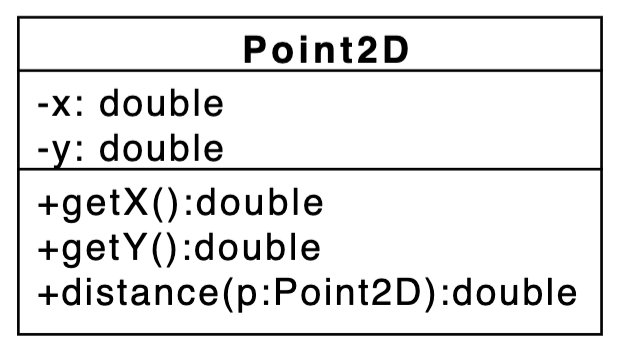
\includegraphics[width=0.5\linewidth]{assets/UML/class/class-1.png}
    \caption{Esempio di definizione di classe}
\end{figure}

\paragraph{Classe} Rappresentata graficamente da rettangoli contenenti almeno il nome della classe e al più le sue caratteristiche. Le caratteristiche (o \textit{feature}) sono divise in \textit{proprietà} e \textit{operazioni}, queste possono avere diversi livelli di visibilità: \textit{public} (+), \textit{private} (-), \textit{protected} (\#) o \textit{package} ($\sim$).

\paragraph{Proprietà} Rappresentano le caratteristiche strutturali di una classe (non temporanee, es. parametri in input di un metodo). Si possono esprimere sotto forma di \textit{attributo}:
\begin{center}
    $\langle$visibilità$\rangle$ $\langle$nome$\rangle$ : $\langle$tipo$\rangle$ $\langle$molteplicità$\rangle$ = $\langle$default$\rangle$ \{$\langle$proprietà$\rangle$\}
\end{center}
Dove:
\begin{itemize}
    \item La \textbf{visibilità} è indicata con un simbolo;
    \item Il \textbf{tipo} indica l'insieme di valori assumibili;
    \item La \textbf{molteplicità} vincola il numero di oggetti che possono costituire l'attributo. Espressa come intervallo $[m, n]$;
    \item Il \textbf{default} è valore predefinito;
    \item La \textit{proprietà} è una stringa che indica vincoli aggiuntivi (es. \textit{read-only} o \textit{frozen}). Per specificare il criterio di l'ordinamento si usano \textit{ordered} o \textit{sorted}
\end{itemize}
Si esprimono \textit{attributi} (il cui tipo è non significativo) e \textit{associazioni} (il cui tipo è significativo, espresso da un'altra classe del sistema).
Non esiste un metodo univoco di traduzione, ma in linguaggi moderni quali Java le proprietà corrispondono ai campi (spesso esposti tramite metodi accessori quali \textit{get} e \textit{set} o \textit{wrapper} per collezioni), mentre le operazioni corrispondono ai metodi.

\subparagraph{Proprietà derivata} È una proprietà per la quale non serve introdurre un campo per memorizzarla e può essere calcolata a partire da altre proprietà, è indicata come attributo accompagnato dal simbolo "$/$" corredato da una nota che esprime come ottenerla. Esprime un vicolo (concetto di \textit{invariante di classe}) per le proprietà coinvolte.

\begin{figure}[H]
    \centering
    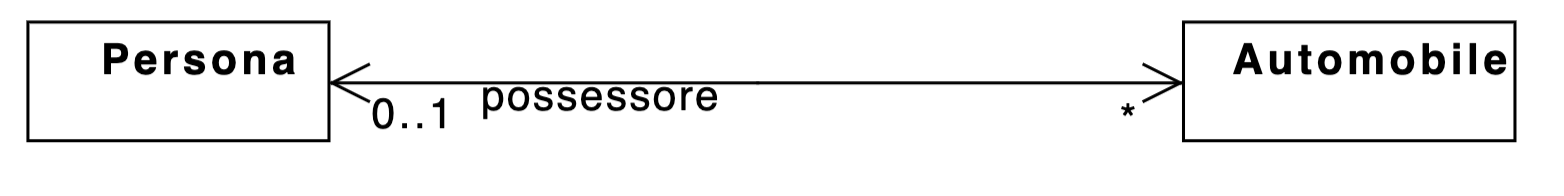
\includegraphics[width=0.75\linewidth]{assets/UML/class/class-3.png}
    \caption{\textbf{Associazione bidirezionale} - ogni oggetto Persona può avere una collezione di oggetti Automobile; ogni oggetto Automobile può avere proprietà opzionale di tipo Persona}
\end{figure}

\paragraph{Operazioni} Rappresentano caratteristiche funzionali delle istanze di una classe (azioni invocabili su di esse). Vengono rappresentate tramite stringhe composte come segue:
\begin{center}
        $\langle$visibilità$\rangle$ $\langle$nome$\rangle$(lista\_parametri) : $\langle$tipo\_ritorno$\rangle$ \{$\langle$proprietà$\rangle$\}
\end{center}
La lista dei parametri va specificata. Ogni parametro è separato da virgole ed è espresso come segue:
\begin{center}
        $\langle$direzione$\rangle$ $\langle$nome$\rangle$ : $\langle$tipo$\rangle$ = $\langle$default$\rangle$
\end{center}
Dove:
\begin{itemize}
    \item La \textbf{direzione} indica se il parametro è in input (\textit{in}), in output (\textit{out}) o entrambi (\textit{inout});
    \item La \textbf{proprietà} indica se l'operazione cambia o meno lo stato del sistema. Se non lo cambia si aggiunge la stringa \textit{query}.
\end{itemize}
Nota: Java non permette di specificare la direzione o valore default dei parametri.
UML distingue operazioni (dichiarazione di una procedura) e metodi (corpo dell'operazione).

\subparagraph{Static} Vengono definiti \textit{static} quegli attributi o quelle operazioni che si riferiscono alla classe e non alle sue istanze. Nel diagramma le caratteristiche \textit{static} vengono sottolineate.

\newpage

\paragraph{Generalizzazione} Anche i class diagram ammettono relazioni di generalizzazione che partono da classi \textit{specializzate} e puntano ad una classe \textit{generale}. In Java viene espressa con il concetto di \textit{ereditarietà} (classe specializzata sottoclasse di classe generica o superclasse - \textbf{Principio di sostituibilità di Liskov}).

\begin{figure}[H]
    \centering
    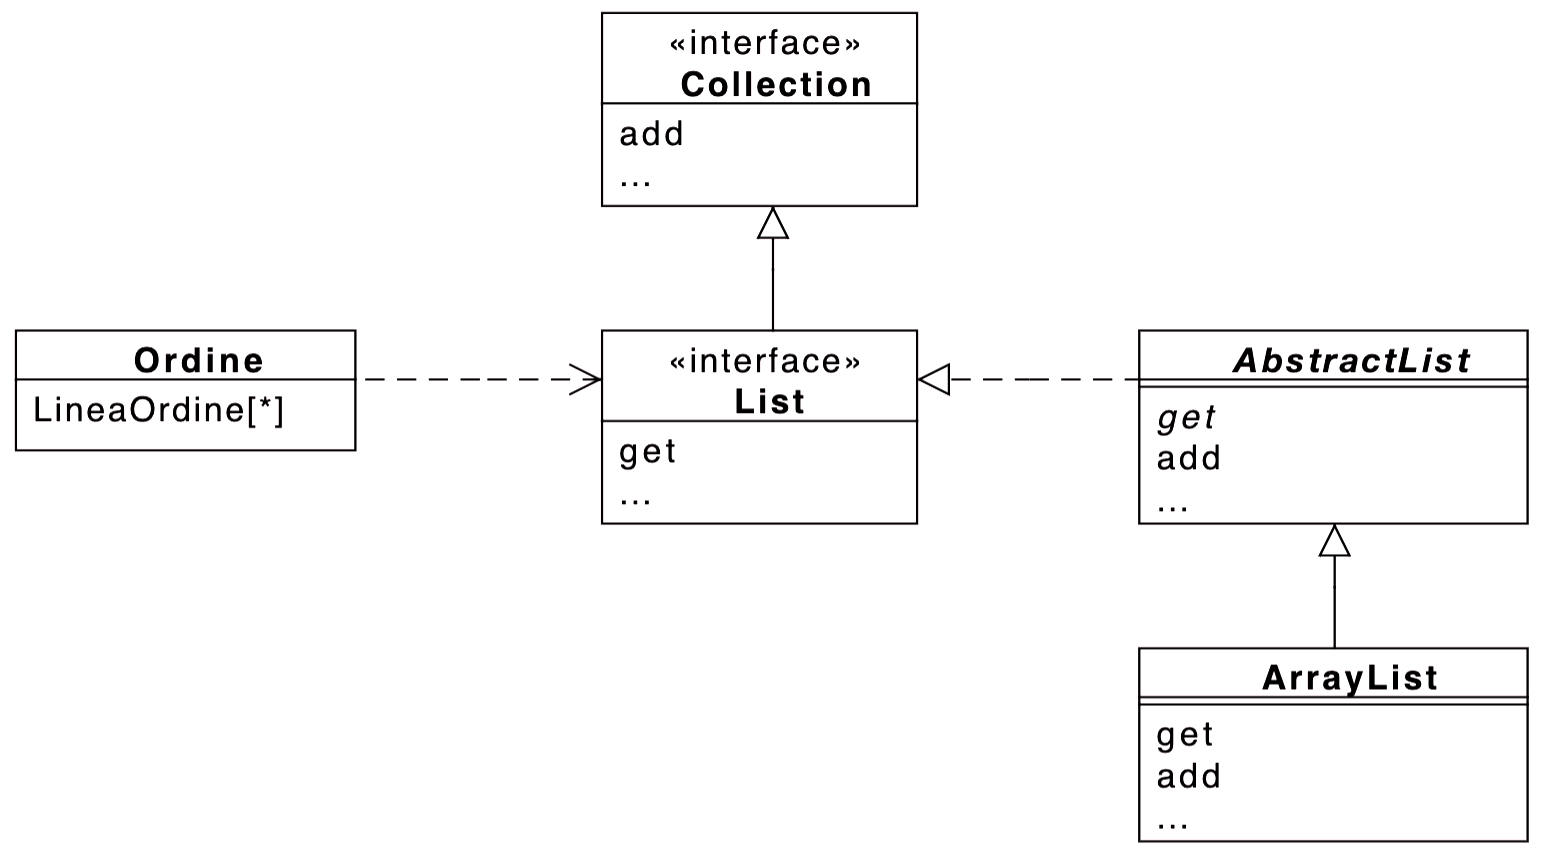
\includegraphics[width=0.75\linewidth]{assets/UML/class/class-8.png}
    \caption{Esempio di generalizzazione}
\end{figure}

Di seguito un esempio in Java che non rispetta il principio di Liskov:
\begin{minted}[
    fontsize=\footnotesize,
    linenos,
]{java}
public class Rettangolo {
    private double base;
    private double altezza;

    public void setBase(double b) { base = b; }
    ...
    public double getBase() { return base; }
    ...
    public double getArea() { return base * altezza; }
}

public class Quadrato extends Rettangolo {
    public Quadrato(double l) {
        super(l, l);
    }
    ...
}
\end{minted}

Sebbene \textit{geometricamente} un quadrato è un rettangolo, l'implementazione è \textbf{sbagliata} in quanto non deve essere possibile sostituire un Quadrato ad un Rettangolo laddove ci si aspetta il secondo. Si hanno quindi due alternative: rendere le classi \textbf{immutabili} o \textbf{separarle}.

I class diagram ammettono il concetto di \textit{classe astratta} (non istanziabile) e \textit{operazione astratta} (solo dichiarata, priva di corpo), convenzionalmente indicate dal nome scritto in corsivo.

È anche possibile definire delle \textit{interfacce} (insieme di operazioni) indicate dalla parola chiave $\langle\langle$interface$\rangle\rangle$.

La relazione che lega interfaccia e classe (astratta o concreta) si dice \textit{realizzazione} e viene rappresentata da una linea tratteggiata con la punta chiusa e vuota che parte dalla classe e punta all'interfaccia.

\begin{figure}[H]
    \centering
    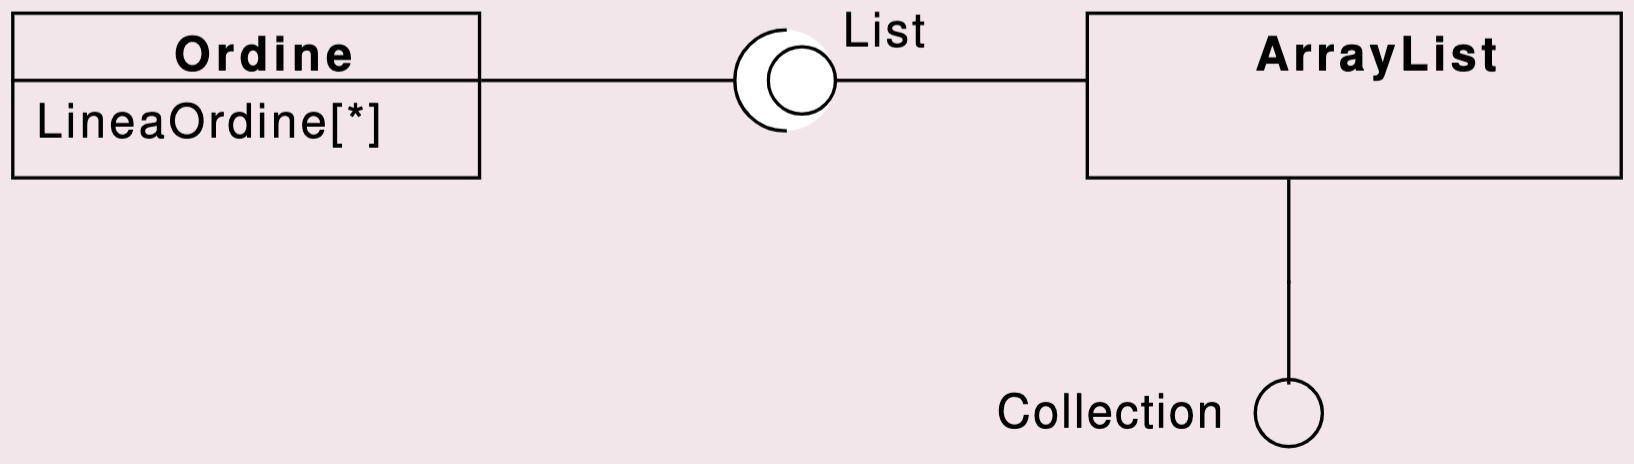
\includegraphics[width=0.75\linewidth]{assets/UML/class/class-9.png}
    \caption{Esempio di utilizzo della notazione \textit{lollipop} (classe fornisce interfaccia) e notazione \textit{socket} (classe richiede interfaccia)}
\end{figure}

\begin{figure}[H]
    \centering
    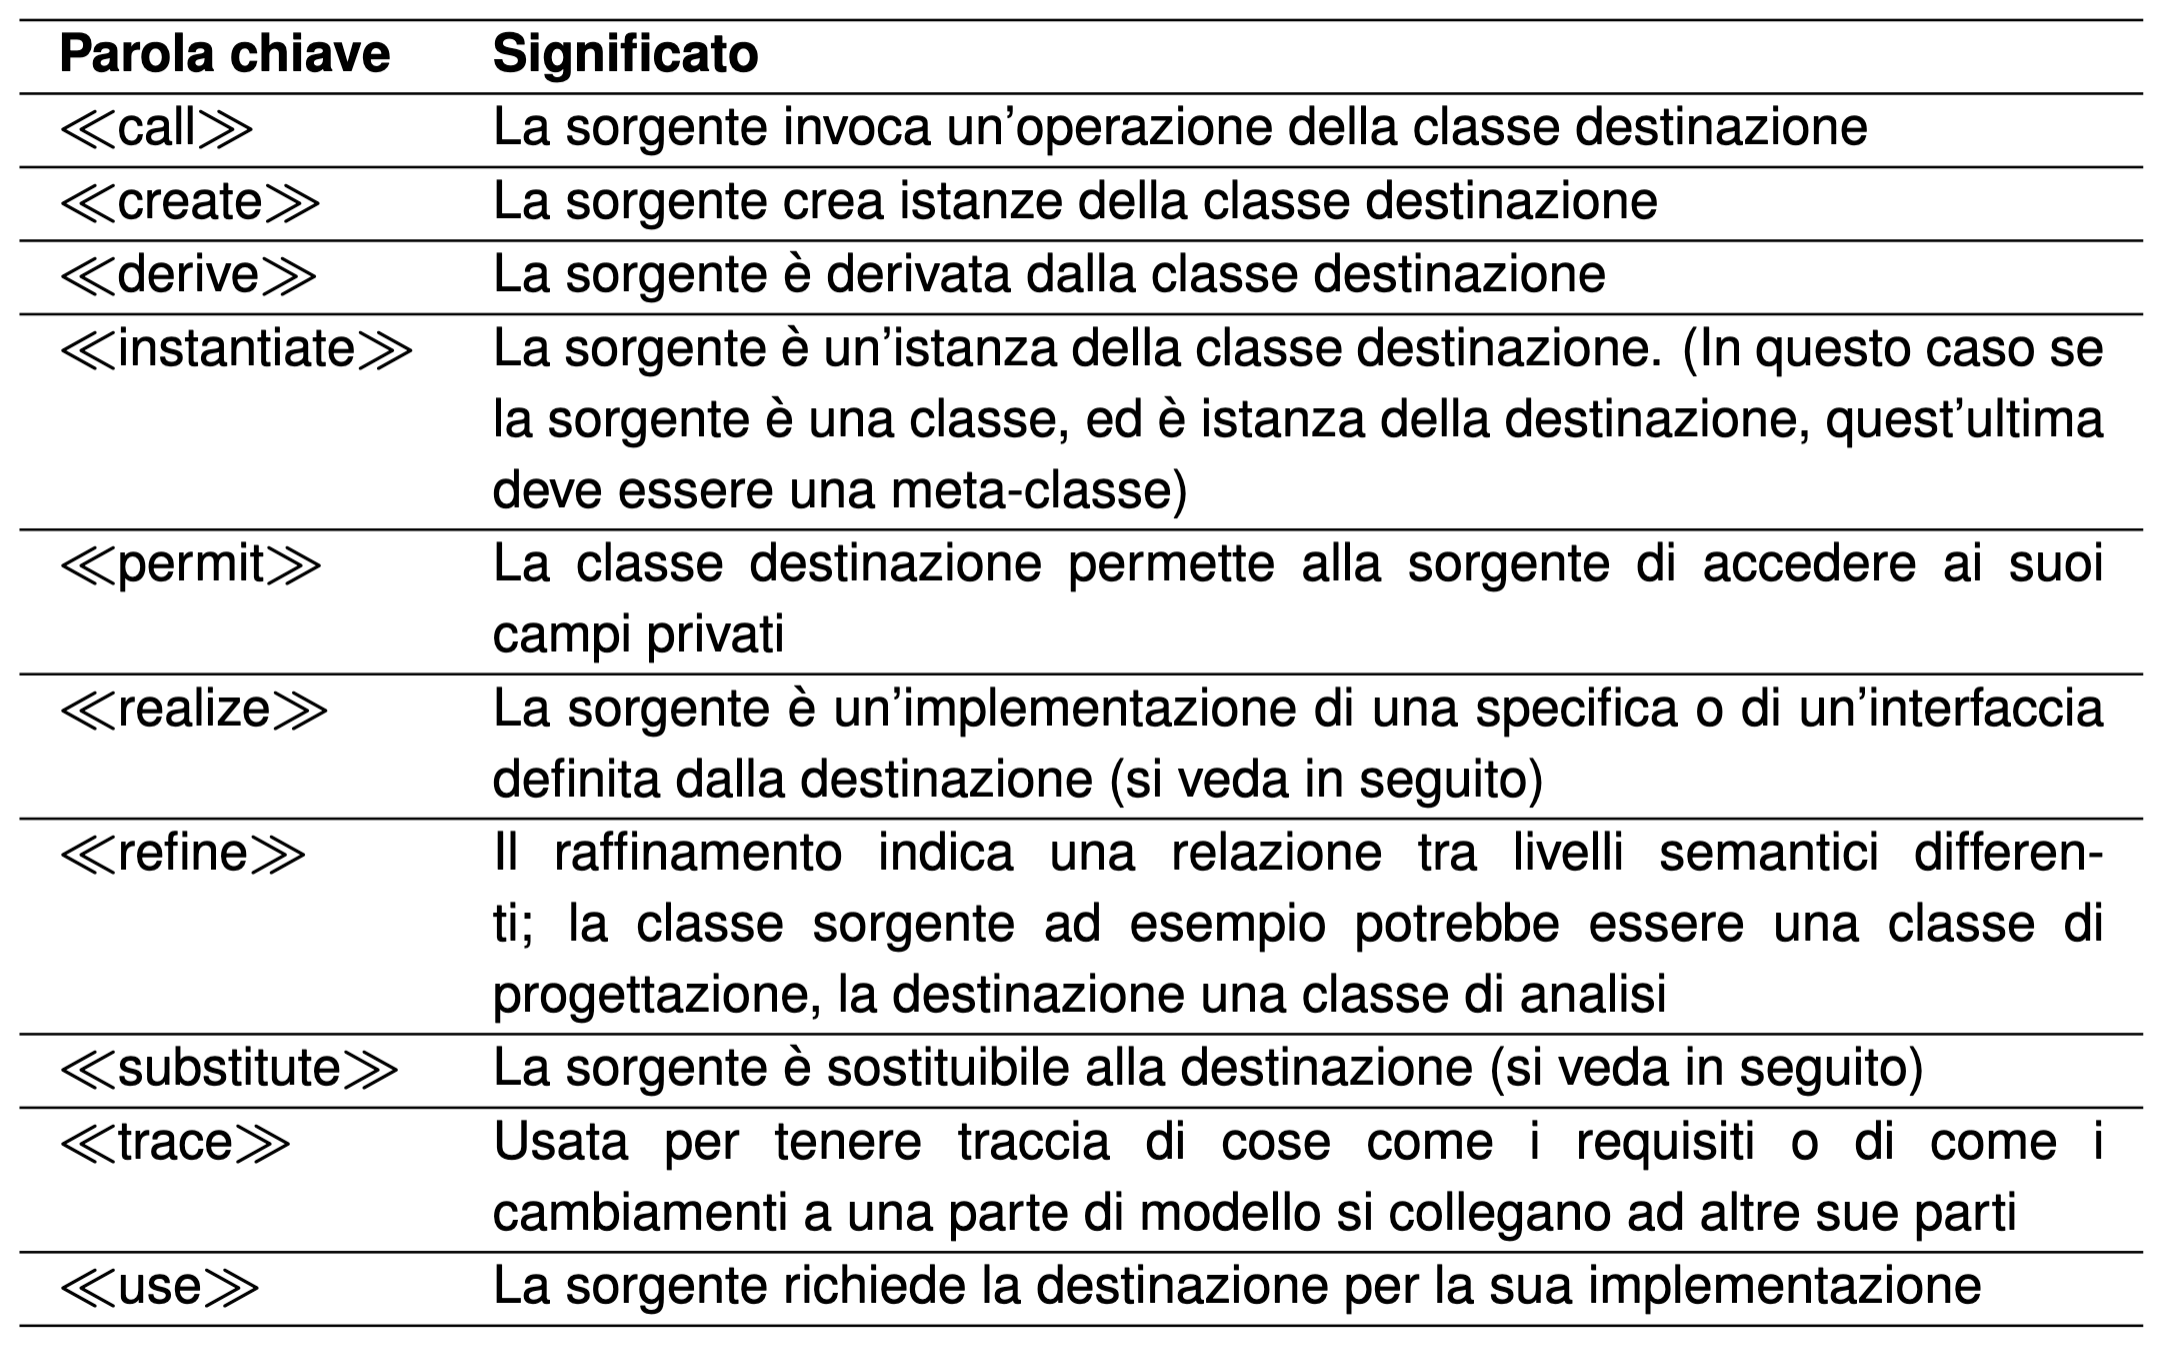
\includegraphics[width=1\linewidth]{assets/UML/class/class-10.png}
    \caption{I class diagram prevedono \textbf{dipendenze}, relazioni unidirezionali tra una classe \textit{client} (da cui parte la freccia) ad una classe \textit{supplier} (in cui punta la freccia). Una qualsiasi modifica alla classe supplier ha effetto sulla classe client (non viceversa), in più NON gode di proprietà transitiva. È inoltre possibile definire dipendenze \textit{custom} (personalizzate)}.
\end{figure}

\begin{figure}[H]
    \centering
    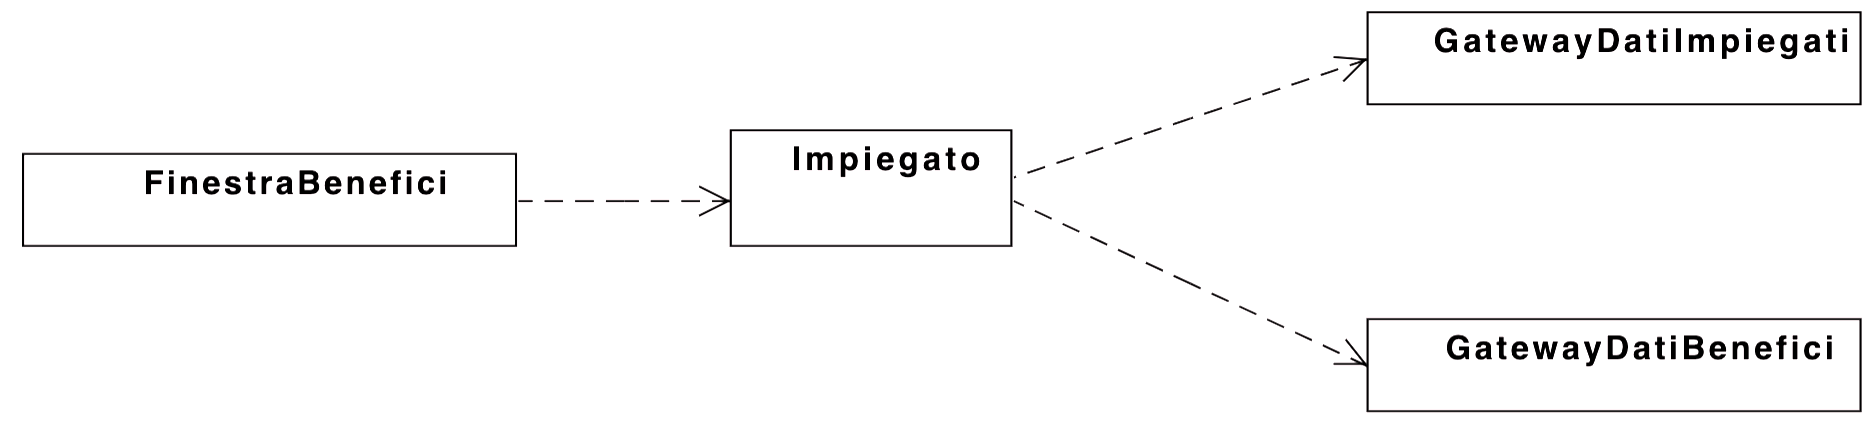
\includegraphics[width=1\linewidth]{assets/UML/class/class-5.png}
    \caption{Esempio di utilizzo del concetto di dipendenza}
\end{figure}

I class diagram consentono l'uso di interfacce e classi \textbf{parametriche}: nel codice, i campi e i parametri/risultati dei metodi sono di tipo generico (sussiste a tempo di compilazione, es. Java) o \textit{template} (sussiste a runtime, es C++).

\begin{figure}[H]
    \centering
    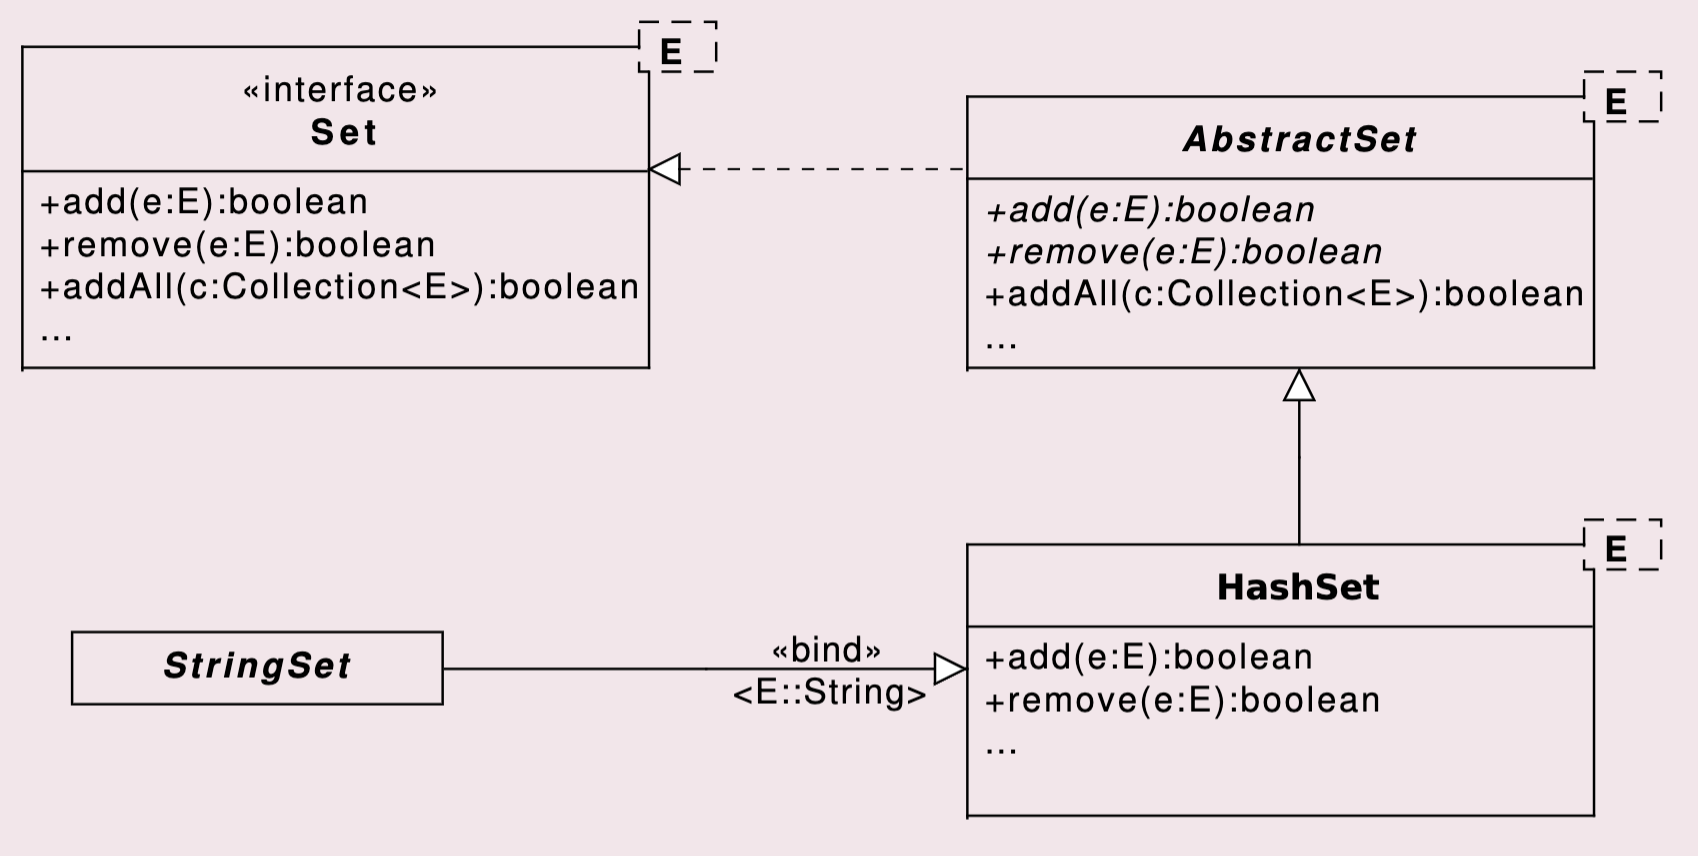
\includegraphics[width=1\linewidth]{assets/UML/class/class-11.png}
    \caption{Esempio di \textbf{derivazione}: classe discendente da una classe parametrica che sostituisce il tipo generico con uno concreto tramite \textit{bind}}
    
\end{figure}
L'introduzione di una classe tramite derivazione fa si che si abbia una relazione di \textit{raffinamento}. 

I tipi che possono assumere solo un set finito di valori prefissati sono modellati tramite \textit{enumerazioni}. 

Una classe \textit{attiva} è una classe che esegue e controlla autonomamente il proprio thread (es. la classe Thread di Java).

\paragraph{Aggregazione} È una forma di associazione in cui l'oggetto destinazione è un \textit{componente} della classe sorgente, il quale viene \textit{aggregato}.

\begin{figure}[H]
    \centering
    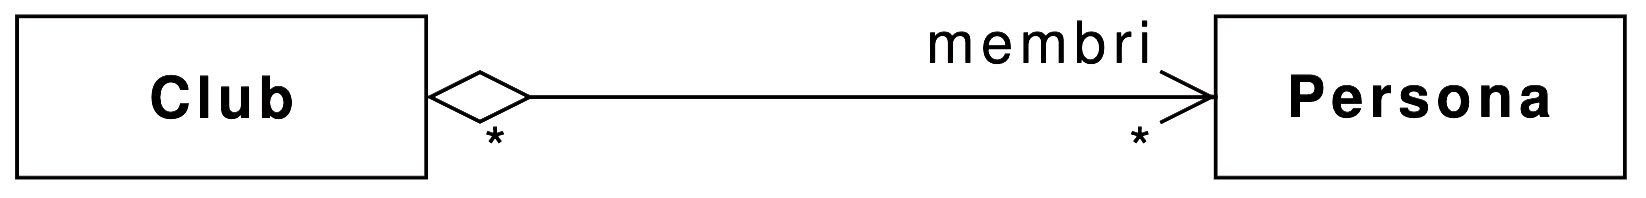
\includegraphics[width=1\linewidth]{assets/UML/class/class-6.png}
    \caption{Esempio di aggregazione}
\end{figure}

\paragraph{Composizione} È una forma di aggregazione in cui l'oggetto sorgente è composto da un insieme di oggetti del tipo destinazione.

\begin{figure}[H]
    \centering
    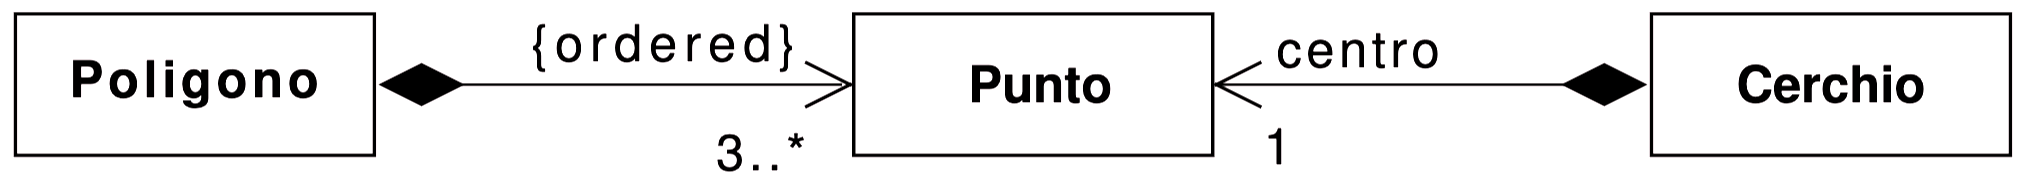
\includegraphics[width=1\linewidth]{assets/UML/class/class-7.png}
    \caption{Esempio di composizione}
\end{figure}
Le differenze tra composizione e aggregazione sono le seguenti:
\begin{itemize}
    \item La \textit{composizione} è una relazione esclusiva: l'oggetto componente può far parte di un solo oggetto composto (uno ad uno); nell'\textit{aggregazione} può esistere una relazione uno a molti.
    \item Nella \textit{composizione}, l'istanza composta è responsabile dell'esistenza (creazione, modifica e cancellazione) delle istanze componenti, se viene distrutta anche i suoi componenti vengono distrutti; nell'\textit{aggregazione} l'oggetto componente esiste in maniera indipendente dall'aggregato.
\end{itemize}

\begin{figure}[H]
    \centering
    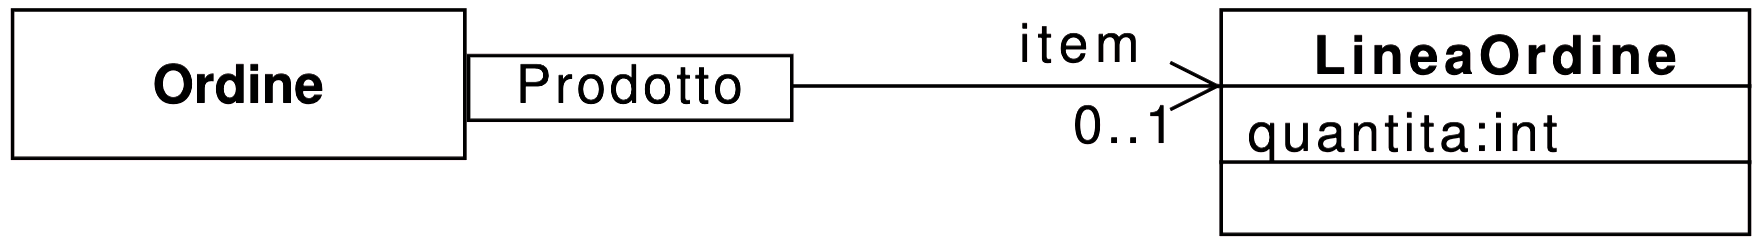
\includegraphics[width=1\linewidth]{assets/UML/class/class-12.png}
    \caption{Esempio di \textbf{associazione qualificata} in cui l'oggetto Ordine possiede più oggetti di tipo LineaOrdine, ma al più uno per ogni oggetto Prodotto (detto \textit{qualificatore}, una sorta di chiave). Implementata tramite array associativi quali mappe, tabelle hash, dizionari, ecc...}
\end{figure}

\vspace{20pt}

\begin{figure}[H]
    \centering
    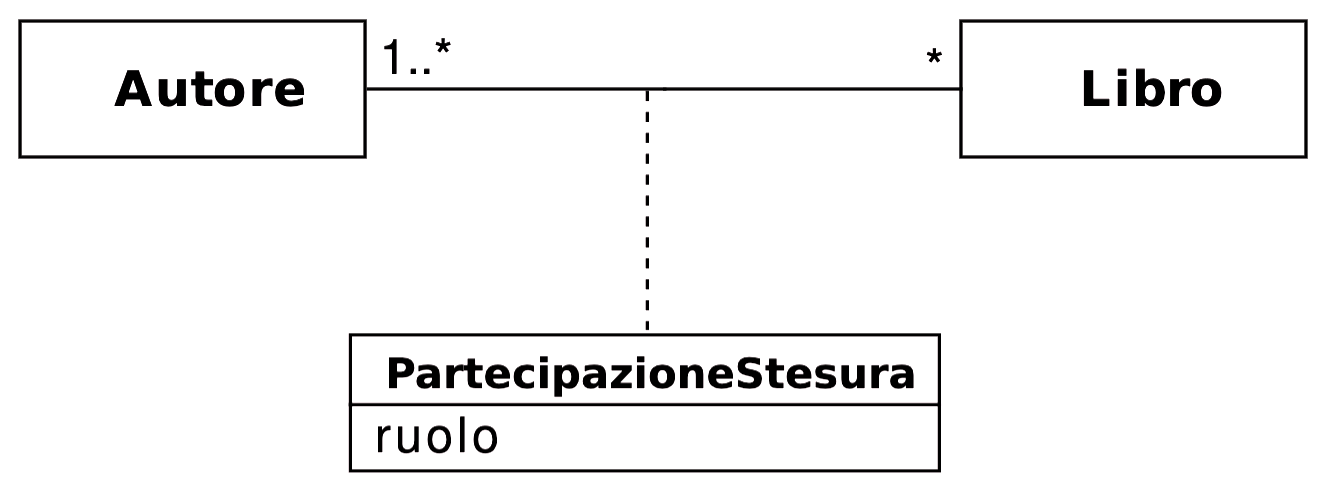
\includegraphics[width=1\linewidth]{assets/UML/class/class-13.png}
    \caption{Esempio di \textbf{classe associativa}: garantisce che per ogni coppia di oggetti associati esista una sola istanza della classe associativa.}
\end{figure}

\vspace{20pt}

\begin{figure}[H]
    \centering
    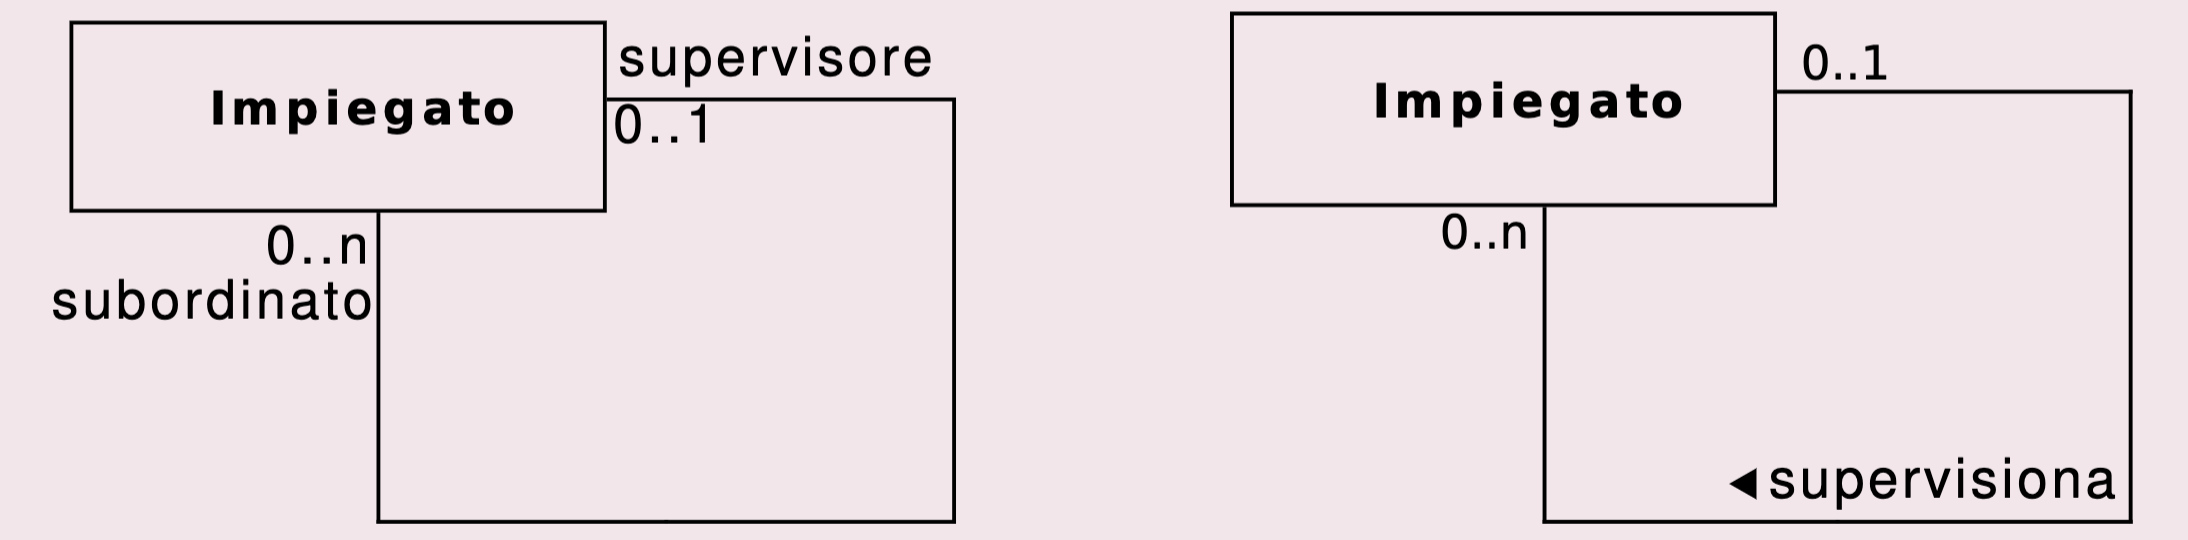
\includegraphics[width=1\linewidth]{assets/UML/class/class-14.png}
    \caption{Esempio di \textbf{associazione riflessiva}: classe sorgente e classe destinazione coincidono, ogni istanza della classe possiede proprietà del suo stesso tipo}
\end{figure}

\vspace{20pt}

\begin{figure}[H]
    \centering
    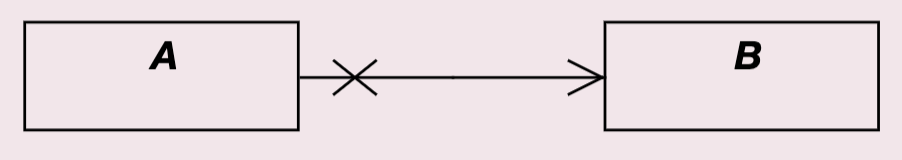
\includegraphics[width=1\linewidth]{assets/UML/class/class-15.png}
    \caption{Concetto di \textbf{non navigabilità}}
\end{figure}

\newpage